\documentclass{beamer}

% select theme
\usetheme{CambridgeUS}
\usecolortheme{beaver}

\usepackage{kotex}
\usepackage{fancyvrb}
\usepackage{color}
\usepackage[mmddyyyy]{datetime}
\usepackage{pythontex}
\usepackage{graphicx, subfigure}

% you need to generate pyg.tex by
% pygmentize -O full -f latex hello.c
% \input{pyg.tex}



% syntax highlighted source code 넣는법:
% http://ubuntuforums.org/showthread.php?t=790610
% pygmentize 명령어가 실행될 수 있도록 하자.
% bash에 그냥 pygmentize라고 치면 어느 패키지를 설치해야 하는지 알려줌.
% then...
% 색깔 명령어가 define될 수 있도록... hello.c를 만든 다음,
% pygmentize -O full -f latex hello.c
% 를 돌리면 무엇을 include해야 하는지, define이 뭐가 필요한지 쭉
% stdout으로 출력해줌.
% pygmentize -f latex hello.c 로 나오는 verbatim문을 긁어붙이면 완성.
\begin{document}

% title slide
\begin{frame}
	\title{합성곱}
	\author{정민우}
	\date{\today}
	\titlepage
\end{frame}



% outline slide
\section*{Outline}
\begin{frame}
\tableofcontents
\end{frame}



\section{전체구조}
\begin{frame}
	완전연결(Fully connected) - Affine 계층
	\begin{figure}
		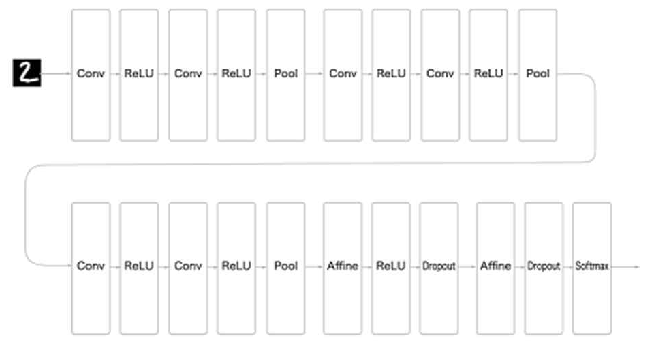
\includegraphics[width=1\columnwidth]{../Figure/Figure_1.pdf}
	\end{figure}
	\begin{figure}
		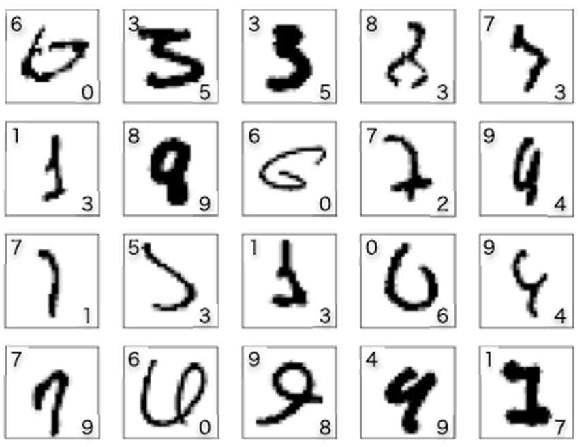
\includegraphics[width=1\columnwidth]{../Figure/Figure_2.pdf}
	\end{figure}	
\end{frame}

\section{합성곱계층}

% 그냥 글자만 있는 슬라이드
% \begin{frame}
% 	\begin{itemize}
% 		\item 합성곱 계층(Convolutional layer)
% 		\item 풀링 계층(Pooling layer)
% 	\end{itemize}
% \end{frame}
% 제목도 들어갔다.
\begin{frame}
	\frametitle{완전연결 계층의 문제점}
	\begin{itemize}
		\item 완전연결계층 : 인접하는 계층의 뉴런이 모두 연결되어 있음
		\item 출력의 수를 임의로 정할 수 있음
		\item 데이터 형상이 무시됨
		\item 3차원 이미지를 1차원 데이터로 바꿔줘야함
		\item 합성곱계층은 형상을 유지함
		\item 특징맵 : 합성곱 계층의 입출력 데이터
	\end{itemize}
\end{frame}

\begin{frame}
	\frametitle{합성곱연산}
	\begin{figure}
		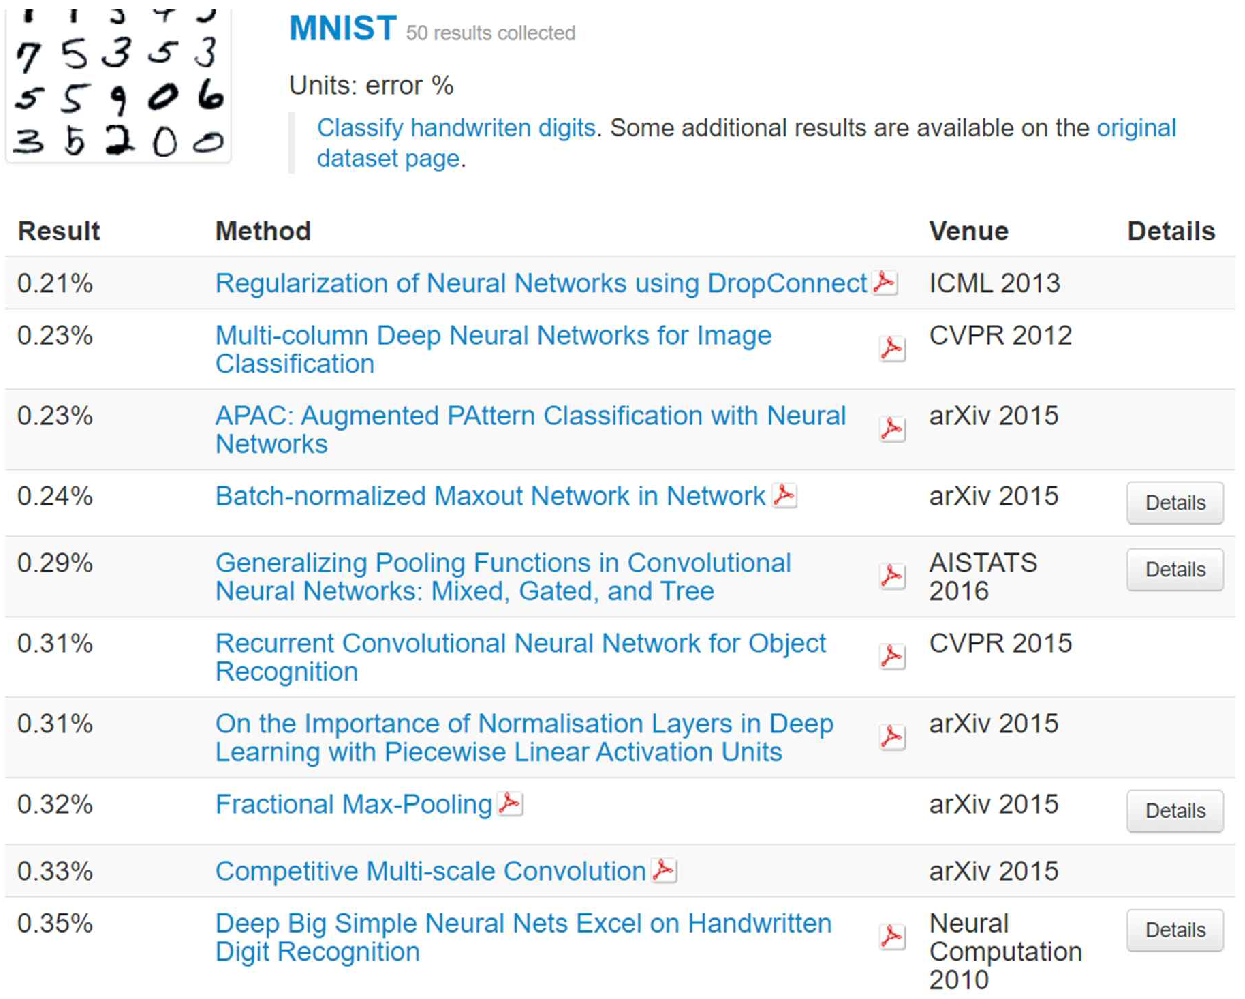
\includegraphics[width=0.45\columnwidth]{../Figure/Figure_3.pdf}
	\end{figure}
\end{frame}

\begin{frame}
	\frametitle{편향(Bias)}
	\begin{figure}
		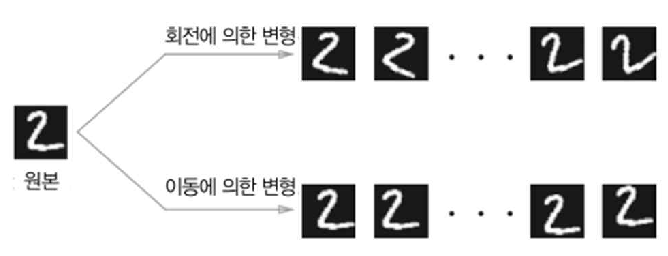
\includegraphics[width=1\columnwidth]{../Figure/Figure_4.pdf}
	\end{figure}
	% \framesubtitle{부제목 넣었다}
\end{frame}
% 부제목이 있는 슬라이드
\begin{frame}
	\frametitle{패딩}
	\begin{itemize}
		\item 정보손실을 막을 수 있음
	\end{itemize}
	\begin{figure}
		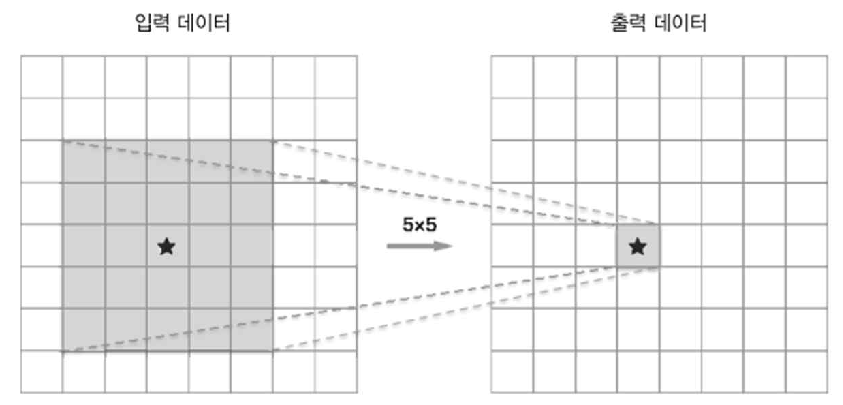
\includegraphics[width=1\columnwidth]{../Figure/Figure_5.pdf}
	\end{figure}
	% \framesubtitle{부제목 넣었다}
\end{frame}

% with bullets
\begin{frame}
	\frametitle{스트라이드}
	\begin{figure}
		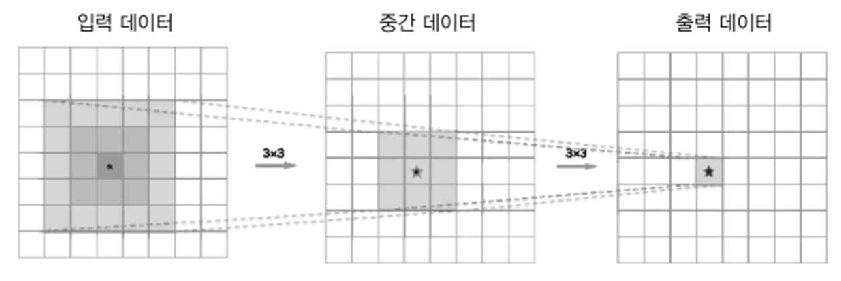
\includegraphics[width=1\columnwidth]{../Figure/Figure_6.pdf}
	\end{figure}
\end{frame}

\begin{frame}
	\frametitle{스트라이드}
	\framesubtitle{출력계산식}
	입력크기 : H,W\\
	필터크기 : FH,FW\\
	출력크기 : OH, OW\\
	$$ OH = \dfrac{H+2P-FH}{S} + 1 $$
	$$ OW = \dfrac{W+2P-FW}{S} + 1 $$
\end{frame}

\begin{frame}
	\frametitle{특징맵 추출 예시}
	\begin{figure}
		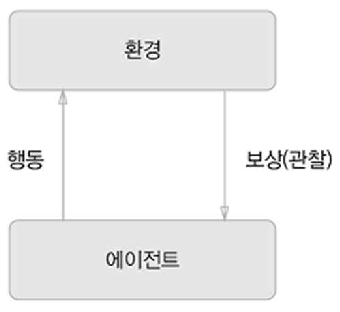
\includegraphics[width=0.5\columnwidth]{../Figure/Figure_16.pdf}
	\end{figure}
\end{frame}

\begin{frame}
	\frametitle{3차원 데이터의 합성곱 연산}
	\begin{figure}
		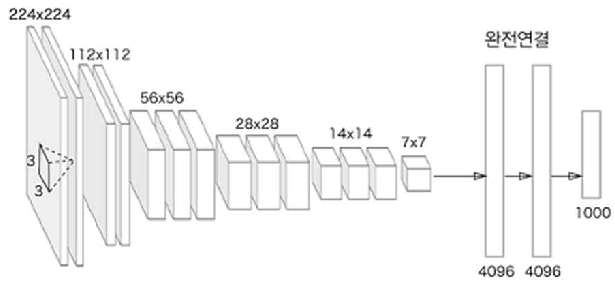
\includegraphics[width=1\columnwidth]{../Figure/Figure_7.pdf}
	\end{figure}
\end{frame}

\begin{frame}
	\frametitle{3차원 합성곱 예시}
	\begin{figure}
		\subfigure{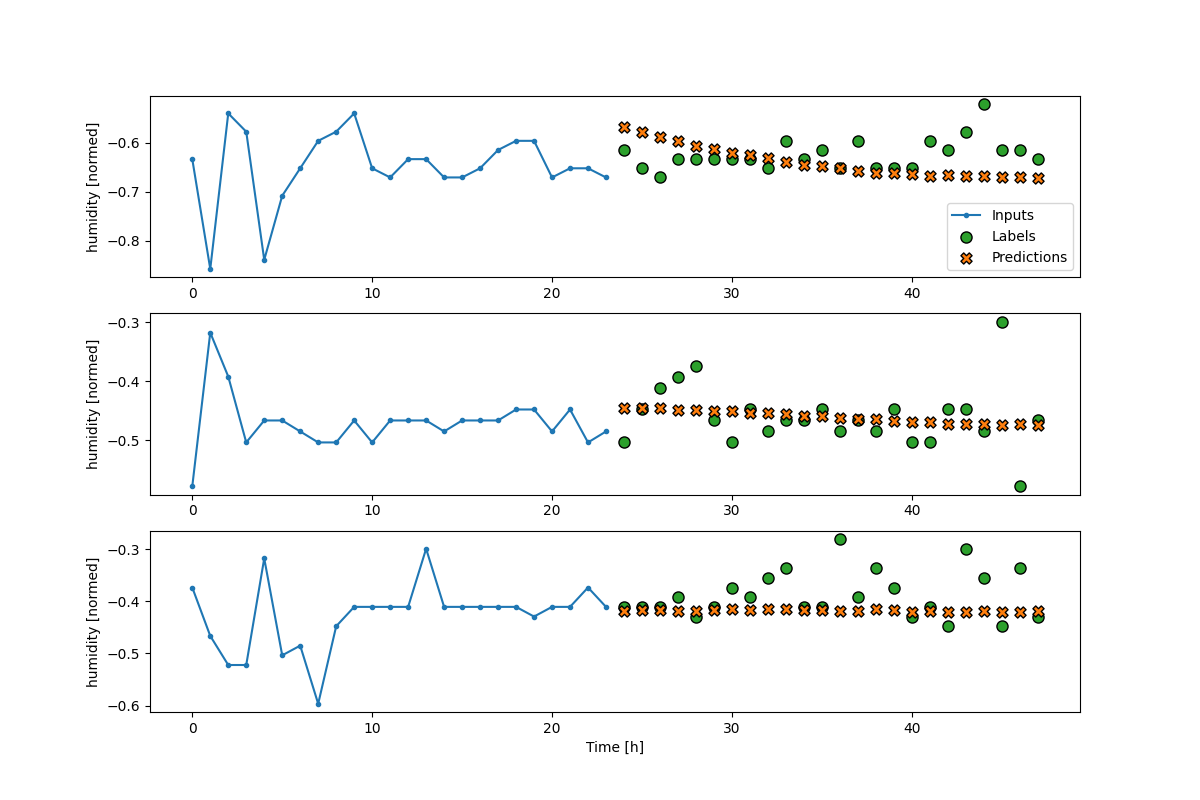
\includegraphics[width=0.4\columnwidth]{../Figure/Figure_18.pdf}}
		\hspace{0.5cm}
		\subfigure{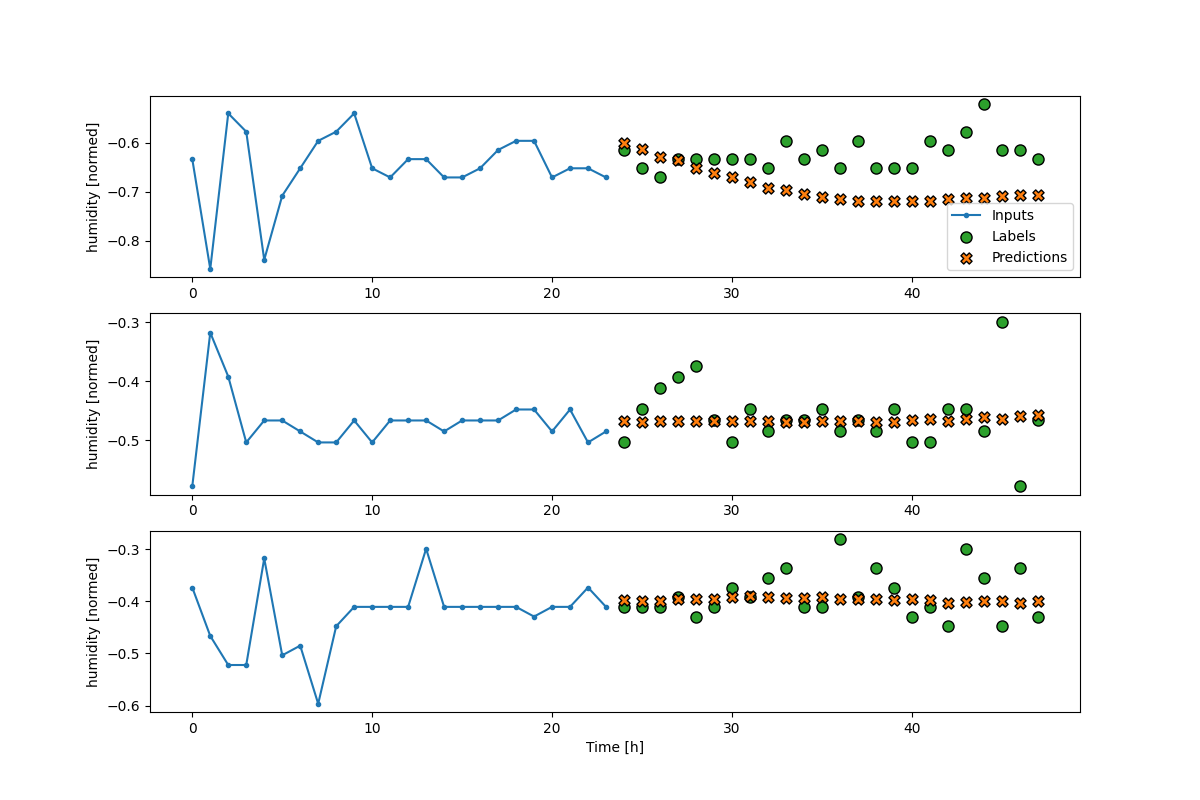
\includegraphics[width=0.5\columnwidth]{../Figure/Figure_19.pdf}}
	\end{figure}
\end{frame}

\begin{frame}
	\frametitle{블록으로 생각하기}
	\begin{figure}
		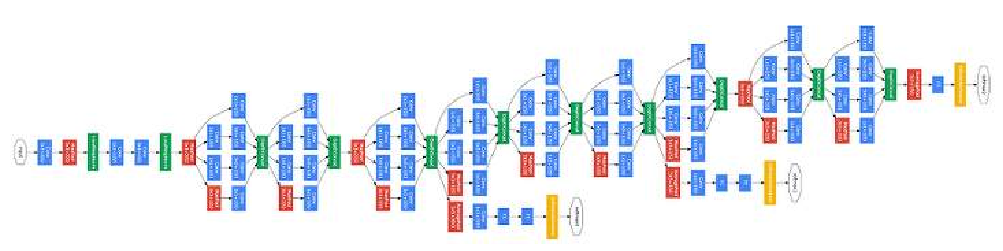
\includegraphics[width=0.8\columnwidth]{../Figure/Figure_8.pdf}
	\end{figure}
\end{frame}

\begin{frame}
	\frametitle{배치처리}
	\begin{figure}
		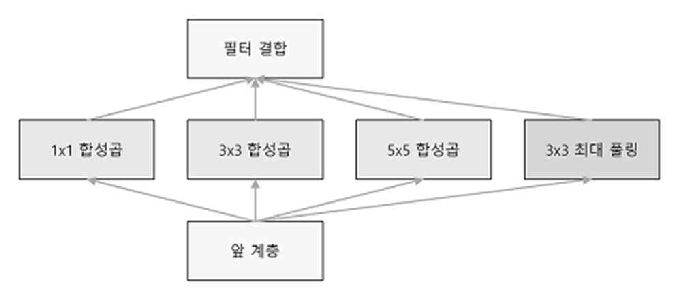
\includegraphics[width=1\columnwidth]{../Figure/Figure_9.pdf}
	\end{figure}
\end{frame}

\section{풀링계층}
	\begin{frame}
		\frametitle{풀링계층}
		\begin{figure}
			\subfigure{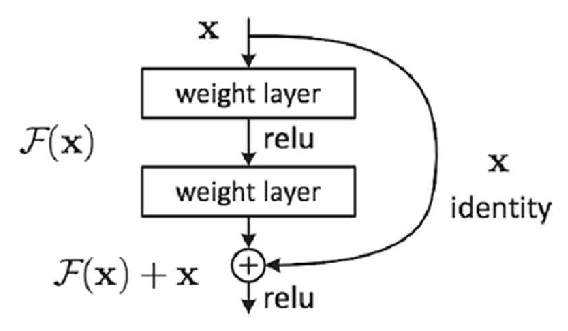
\includegraphics[width=0.6\columnwidth]{../Figure/Figure_10.pdf}}
			% \vspace{0.5cm}
			\subfigure{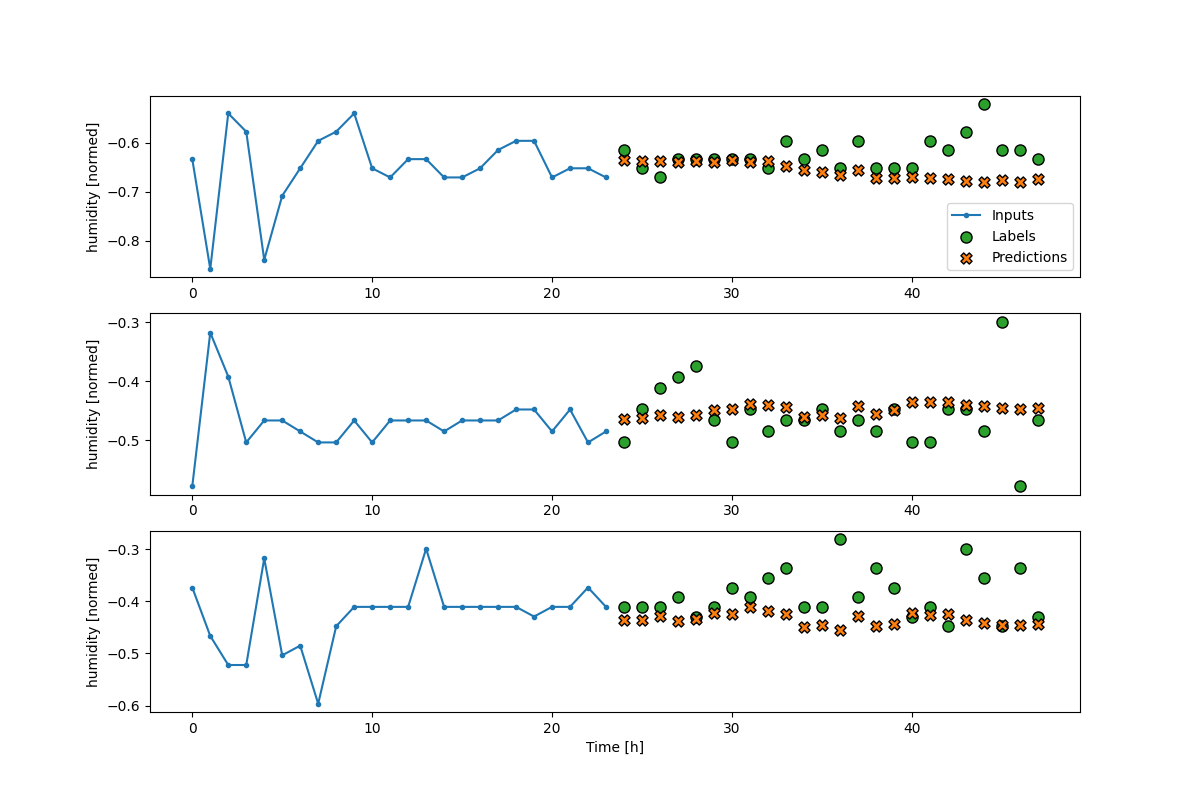
\includegraphics[width=0.6\columnwidth]{../Figure/Figure_17.pdf}}
		\end{figure}
\end{frame}

\begin{frame}
	\frametitle{풀링계층의 특징}
		\begin{itemize}
			\item 학습해야 할 매개변수가 없음
			\item 채널 수가 변하지 않음
			\item 오버피팅을 줄여줌
			\begin{figure}
				\subfigure{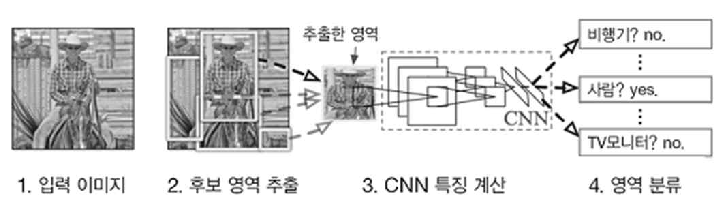
\includegraphics[width=0.5\columnwidth]{../Figure/Figure_11.pdf}}
				% \hspace{0.8cm}
				\subfigure{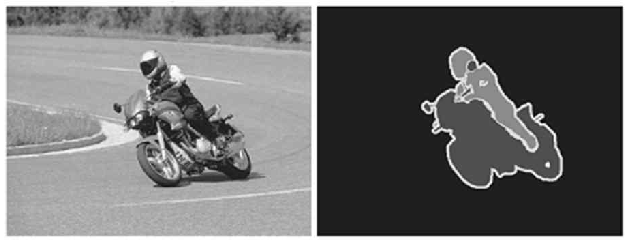
\includegraphics[width=0.6\columnwidth]{../Figure/Figure_12.pdf}}
			\end{figure}
		\end{itemize}
\end{frame}

\section{합성곱/풀링 계층 구현하기}
\begin{frame}
	\frametitle{im2col로 데이터 전개하기}
		\begin{itemize}
			\item 'image to column'
			\item 입력데이터를 필터링하기 좋게 전개하는 함수
			\item 3차원 입력데이터 $\rightarrow$ 2차원 행렬
			\item 메모리 사용량이 증가함

			% \begin{figure}[H!]
			% 	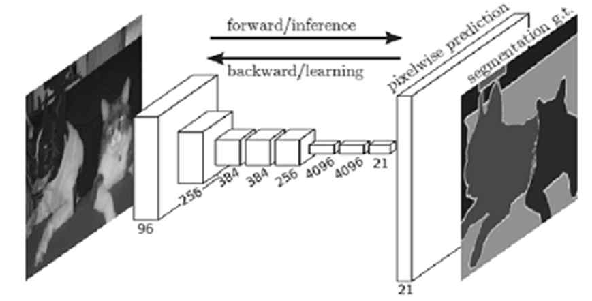
\includegraphics[width=0.3\columnwidth]{../Figure/Figure_13.pdf}
			% \end{figure}
			% \begin{figure}[H!]
			% 	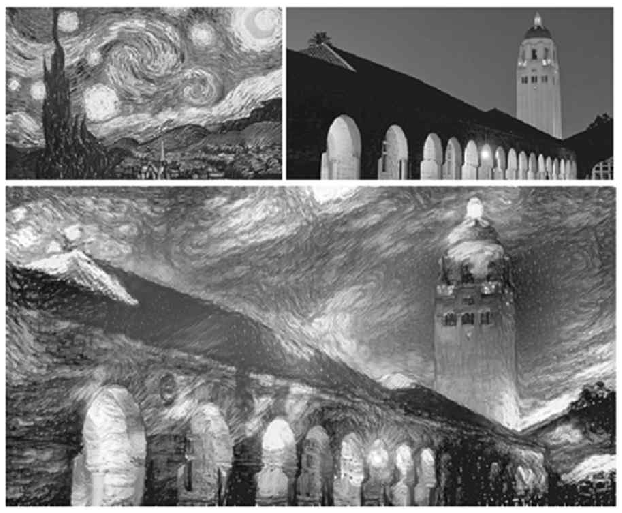
\includegraphics[width=0.3\columnwidth]{../Figure/Figure_14.pdf}
			% \end{figure}

			\begin{figure}
				\subfigure{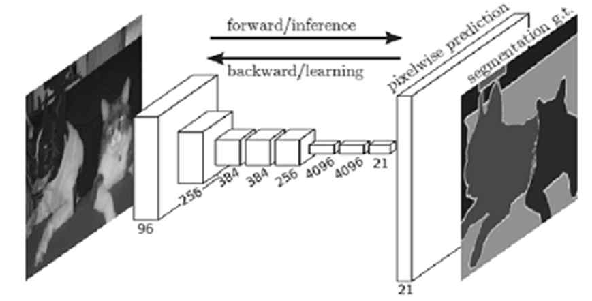
\includegraphics[width=0.3\columnwidth]{../Figure/Figure_13.pdf}}
				\hspace{0.8cm}
				\subfigure{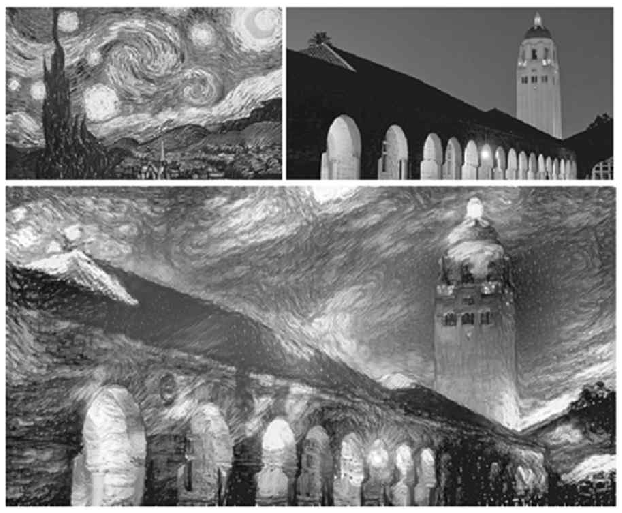
\includegraphics[width=0.3\columnwidth]{../Figure/Figure_14.pdf}}
				\subfigure{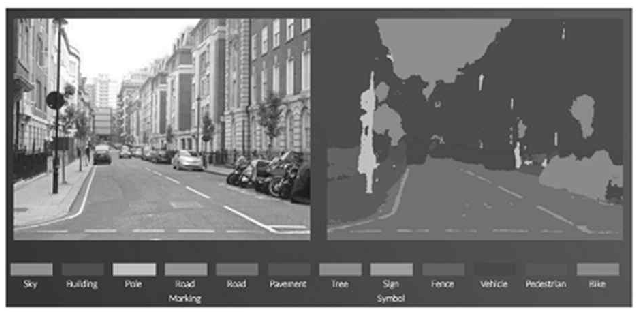
\includegraphics[width=0.4\columnwidth]{../Figure/Figure_15.pdf}}
			\end{figure}
		\end{itemize}
\end{frame}

\begin{frame}
	\frametitle{Train}
		% \begin{itemize}
		% 	\item 'image to column'
		% 	\item 입력데이터를 필터링하기 좋게 전개하는 함수
		% 	\item 3차원 입력데이터 $\rightarrow$ 2차원 행렬
		% 	\item 메모리 사용량이 증가함
			\begin{figure}
				\subfigure{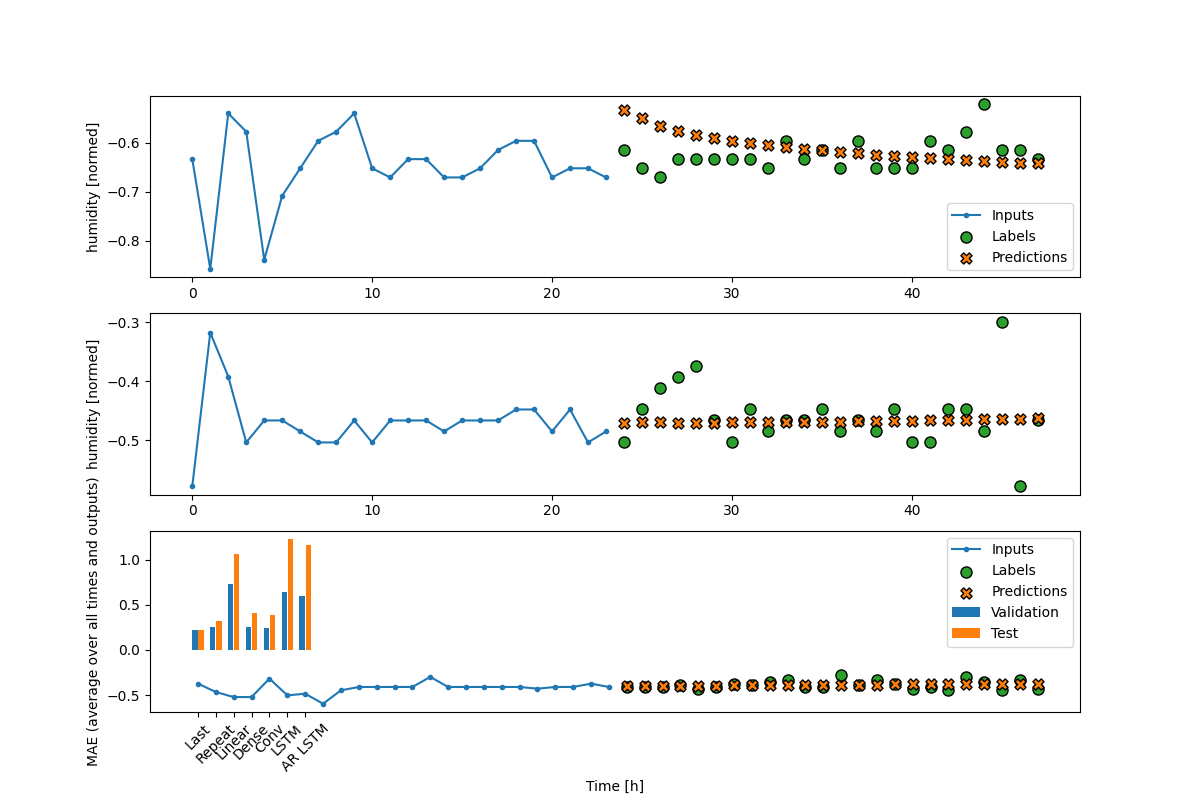
\includegraphics[width=0.5\columnwidth]{../Figure/Figure_20.pdf}}
				\hspace{0.8cm}
				\subfigure{\includegraphics[width=0.4\columnwidth]{../Figure/Figure_21.pdf}}
				% \subfigure{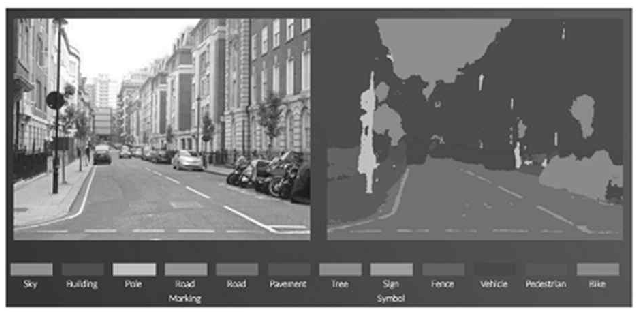
\includegraphics[width=0.4\columnwidth]{../Figure/Figure_15.pdf}}
			\end{figure}
		% \end{itemize}
\end{frame}
% \begin{frame}
% 	\frametitle{4차원 배열}

	% \begin{pycode}
	% 	print("Hello Python")
	% \end{pycode}

	% \begin{pyconsole}
	% 	x = np.random.rand(10,1,28,28)
	% 	x.shape
	% \end{pyconsole}

	% \begin{pycode}
	% 	x = np.random.rand(10,1,28,28)
	% 	x.shape
	% 	x[0].shape
	% 	x[1].shape
	% \end{pycode}
% \end{frame}

\end{document}

% \begin{frame}
% 	\begin{figure}
% 	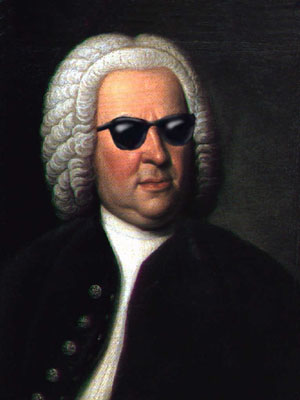
\includegraphics[width=0.3\columnwidth]{jpg/bach_shades.jpg}
% 	\end{figure}
% 	그림 넣은 슬라이드 \\
% 	``It's easy to play any musical instrument: all you have to do is touch the right key at the right time and the instrument will play itself.''
% 	\footnote{\url{http://thinkexist.com/quotation/it-s_easy_to_play_any_musical_instrument-all_you/13822.html}}
% \end{frame}

% \begin{frame}
% 	\frametitle{칼럼 넣은 슬라이드}
% 	\begin{columns}
% 	\begin{column}{0.5\textwidth}
% 		\begin{figure}
% 		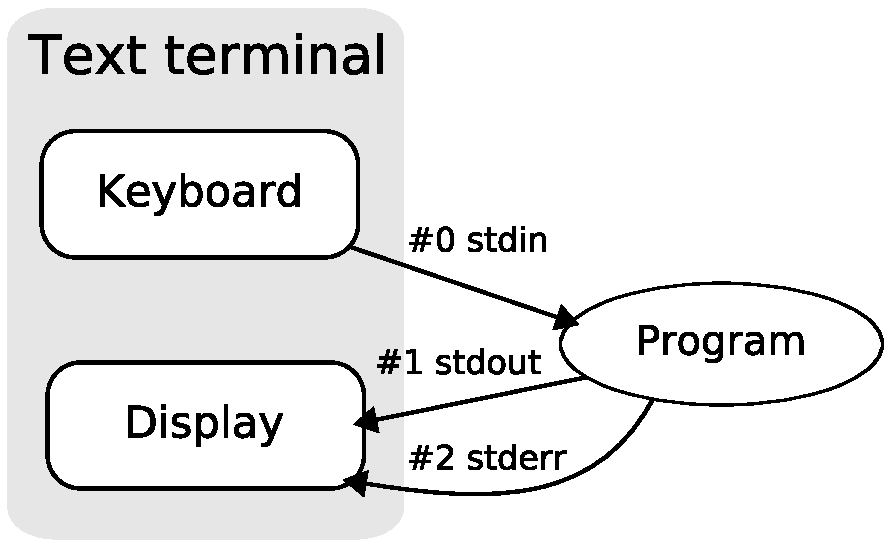
\includegraphics[width=0.9\columnwidth]{svg/Stdstreams-notitle}
% 		\end{figure}
% 	\end{column}
% 	\begin{column}{0.5\textwidth}
% 		\begin{itemize}
% 			\item stdout
% 			\item stderr
% 			\item stdin
% 		\end{itemize}
% 	\end{column}
% 	\end{columns}
% \end{frame}

% \begin{frame}[fragile] % Verbatim을 썼으므로 fragile표시를 해줘야 함.
% 	\frametitle{코드를 넣은 슬라이드}
% 	다음은 Hello World! 프로그램이다.
% 	c/pyg.sh hello.c 를 하면 나오는 내용을 여기 붙이면 되는 것임.
% \begin{Verbatim}[commandchars=\\\{\}]
% \PY{c+cp}{#}\PY{c+cp}{include <stdio.h>}

% \PY{k+kt}{int} \PY{n+nf}{main}\PY{p}{(}\PY{p}{)}
% \PY{p}{\PYZob{}}
%         \PY{n}{fprintf}\PY{p}{(} \PY{n}{stderr}\PY{p}{,} \PY{l+s}{"}\PY{l+s}{Program terminated with error!}\PY{l+s+se}{\PYZbs{}n}\PY{l+s}{"} \PY{p}{)}\PY{p}{;}
%         \PY{k}{return} \PY{l+m+mi}{1}\PY{p}{;}
% \PY{p}{\PYZcb{}}
% \end{Verbatim}
% \end{frame}

% \subsection{서브섹션을 가르면 진도표에 반영됨}

% \begin{frame}
% 	\frametitle{Caeser Cypher II}
% 	{\em \Large Practice1 - Caeser Cypher II}

% 	\vspace{5mm}
% 	중간 타이틀로서 나름 깔끔한듯.
% 	part기능에는 좀 어울리지 않아서 손으로 직접... 읔;;
% \end{frame}

% \section{다른 섹션}

% \begin{frame}[containsverbatim]
% 	\frametitle{그냥 verbatim}
% 	터미널의 출력 따위
% 	\begin{verbatim}
% 	$ chmod -x a.out
% 	$ chmod +x a.out
% 	$ chmod -r test.c
% 	$ chmod +r test.c
% 	$ chmod -w test.c
% 	$ chmod +w test.c
% 	\end{verbatim}
% \end{frame}

% \subsection{Practice2 - chmod}

% \begin{frame}
% 	\frametitle{Practice2 - chmod}
% 	{\em \Large Practice2 - chmod}

% 	\vspace{5mm}
% 	set, unset, get 함수를 완성하여 chmod를 따라해보자.
% 	set, unset, get함수에는 if문이 필요 없다.
% \end{frame}

